\chapter{Game and AI Implementation}

The primary objective of this study is to design and develop a framework for the implementation and evaluation of artificial intelligence (AI) agents in Durak. Since the framework in this game is tailored to support the application and evaluation of AI algorithms within the game environment, the focus of this chapter is to provide a high-level overview of the framework's architecture, including its capabilities for supporting the development and evaluation of AI agents for Durak.

\section{OS support}

I tested the game framework for Durak on both the Windows 10 and Linux operating systems to confirm compatibility and functionality. While this list is not exhaustive, and the framework may potentially run on other operating systems, these are the only ones that were formally tested.

\section{A High-Level View of the Framework}

The Durak AI framework includes a game model, AI agents, and a command-line interface (CLI) that are implemented using the C\# programming language and targeted for the .NET 6 platform.

In order to run and test the program, the project has to be cloned from the repository . The source code for the project is available on the project GitHub page \citep{DurakRepo}. From the CLI directory of the project, the user can use the command line to enter the following command: 
\begin{lstlisting}
$ dotnet run
\end{lstlisting}
This will launch the command-line interface and provide guidance on how to proceed with experimentation (for additional information, please refer to Section \ref{CLI}).

An analysis of the source code using Visual Studio's Calculate Code Metrics for Solution feature revealed that the solution consists of a total of 3034 lines of source code. This includes 993 lines in the Agent project, 757 lines in the CLI project, and 1284 lines in the game model.

\subsection{Project Structure}
The game Durak is organized within a solution file, with the file extension ``.sln'', which is a type of file used to manage projects in Visual Studio. This solution includes three individual projects: 

\begin{itemize}

\item \textbf{Model} - A C\# library project that contains the game logic for Durak.

\item \textbf{Agent} - A C\# library that contains all of the implemented AI agents.

\item \textbf{CLI} - A C\# Command-Line Interface (CLI) project that includes parameters for modifying the game model and agents settings in order to perform experiments.

The aforementioned components will be further discussed in the following subsections.

\end{itemize}

\subsection{Model}

The game model, which represents the current state of the game, is implemented using object-oriented programming principles. As was mentioned before, the game logic for Durak is contained within the \textbf{Model} C\# library, which serves as a modular and reusable unit. It includes class objects, such as \texttt{Player}, \texttt{Card}, and \texttt{Deck}, as well as all of the other main components that make up the game. 

\begin{figure}[h]
    \centering
    \captionsetup{justification=centering}
    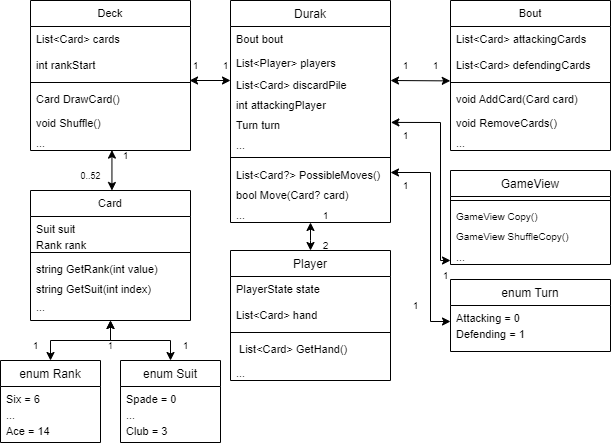
\includegraphics[width=0.9\textwidth]{../img/modelUML.png}
    \caption{A simplified UML diagram showing the relationship between the objects within the Model library.}
    \label{fig:modelUML}
\end{figure}

Before delving into the description of the game state and components of Durak, it is useful to first consider the relationship of all of the objects in the model to that state. A class diagram illustrating the relationships between the objects in the model can be found in Figure \ref{fig:modelUML}.

The \texttt{Deck} object includes the property \texttt{rankStart}, which is an integer value that can be modified from the command-line to alter the starting rank of the cards in the deck. By default, the \texttt{rankStart} is set to 6, but it can be changed to any value between 6 and 14. For instance, if the \texttt{rankStart} is set to 13, the deck will only consist of 8 cards: 4 Aces (rank value 14) and 4 Kings (rank value 13). 

The representation of the game state \texttt{Durak} in the model is a key aspect of the overall system. This representation holds all of the necessary information and logic required to play the game of Durak, shown in Figure \ref{fig:codeDurak}, and therefore plays a central role in the functioning of the model. As such, it is important to carefully consider the design and implementation of the game state representation along with its components. 

\begin{figure}[h]
\captionsetup{justification=centering}
\begin{lstlisting}
// Bout object of the game
private Bout bout;

// Deck object of the game
private Deck deck;

// Trump card of the game that can be assigned or not
private Card? trumpCard;

// Representation of the discard pile in the game
private List<Card> discardPile = new List<Card>();

// Players inside the game
private List<Player> players = new List<Player>();

\end{lstlisting}
\caption{A simplified diagram of the Durak class, which encompasses the main properties of the game}
\label{fig:codeDurak}
\end{figure}

The object in question serves as a comprehensive representation of all game states and data throughout a single game of Durak. To facilitate communication and coordination between the Durak model and the agents that interact with it, the game state provides two primary functions: \texttt{PossibleMoves}, shown in Figure \ref{fig:codePossibleMoves} and \texttt{Move}, shown in Figure \ref{fig:codeMove}. These functions serve as the primary means of interaction between agents and the game state, and as such, play a crucial role in the overall operation of the model. 

\begin{figure}[h]
\captionsetup{justification=centering}
\begin{lstlisting}
if (turn == Turn.Attacking){
    if (CanAttack() && OpponentCanFitMoreCards()) {
        return GenerateListOfAttackingCards();
    } else {
        // passing the attack
        return null;	
    }
}
else {
    Card attackingCard = bout.GetAttackingCards()[^1]
    if (CanDefend(attackingCard)) {
        return GenerateListofDefendingCards(attackingCard);
    } else {
        // taking the cards
        return null
    }
}
\end{lstlisting}
\caption{A simplified overview of the PossibleMoves method inside the Durak class}
\label{fig:codePossibleMoves}
\end{figure}

The \texttt{PossibleMoves} method determines the list of actions that are available to the current player based on the current game state and the rules of the game. When it is the attacker's turn, the method considers the rules for attacking (details in section \ref{attackconditions}) and generates a list of eligible cards that can be played or allows the player to pass if no suitable cards are available. Similarly, when it is the defender's turn (details in section \ref{BeatingRule}), the method takes into account the card being attacked and generates a list of cards that can be played to defend or offers the option to take the attack if no suitable defense is available. Because of that the \texttt{PossibleMove} function returns \texttt{List<Card?>} type. If there are possible moves that can be made in the current state, the function returns a list of the available cards to play. If no moves can be made, the function returns a list containing a single \texttt{null} element, which indicates that the current player must pass or take the card or cards from the bout, depending on the current turn. It should be noted that the example provided in Figure \ref{fig:codePossibleMoves} is a simplified version that omits certain implementation details, such as the process of adding elements to the list. 

\begin{figure}[h]
\captionsetup{justification=centering}
\begin{lstlisting}
if (!ValidAction(card, attacker, defender)) 
    return false;
	
if (turn == Turn.Attacking){
    if (card is not null) {
        attacker.GetHand().Remove(card);
        bout.AddCard(card);
    } else {
        bout.RemoveCards();
        return true;
    }
}
else {
    if (card is not null){
        defender.GetHand().Remove(card);
        bout.AddCard(card);
    } else {
        FillPlayerHand(bout.GetEverything(), defender)
        return true;
    }	
}
turn = turn == Turn.Attacking ? Turn.Defending : Turn.Attacking;
return true;
\end{lstlisting}
\caption{A simplified overview of the Move method inside the Durak class}
\label{fig:codeMove}
\end{figure}

The \texttt{Move} method modifies the current game state by executing the action chosen by the current player. This move is selected by the agent, which performs calculations based on the possible moves generated by the \texttt{PossibleMoves} method. The specific nature of these calculations depends on the type of agent being used. For example, a rule-based agent may simply select the lowest value rank card, while a more sophisticated agent, such Monte-Carlo Tree Search (MCTS), may use more complex decision-making processes to determine the optimal move to make. Regardless of the type of agent being used, the \texttt{Move} method ultimately updates the game state to reflect the chosen action and advances the game to the next turn. To implement the desired changes, the \texttt{Move} method accepts a parameter of type \texttt{Card?}. This parameter represents the move made by the agent, which can be a card play (type \texttt{Card}), or a pass or draw (type \texttt{null}), depending on the role of the agent. Also, it is worth noting that the \texttt{Move} method returns a boolean value. In order to prevent invalid moves, the method verifies the validity of the intended action before making any changes. If the action is deemed valid, the method returns true; otherwise, it returns false.

Additionally, it is important to note that, for efficiency and security purposes, the agents are not provided with the entire \texttt{Durak} object. One reason is that the Durak class contains a large amount of data and methods that are not relevant to the agents' decision-making process. By providing a smaller class such as \texttt{GameView} that only includes the necessary information, such as methods outlined in Figures \ref{fig:codePossibleMoves} and \ref{fig:codeMove}, the agents can more efficiently access the information they need and ignore the rest. Another reason is that the Durak class contains sensitive or proprietary information that should not be shared with the agents. By using a smaller class such as \texttt{GameView} to provide the necessary information, it is possible to control what information is exposed to the agents and protect any sensitive data.

Other than \texttt{PossibleMoves} and \texttt{Move} methods, the \texttt{Copy} method is an important feature of the \texttt{GameView} object worth mentioning. This method creates a duplicate of the current game state, which is useful for game tree exploration by agents such as Minimax and MCTS, due to their need to examine multiple potential moves and outcomes. For further information on the use of the \texttt{Copy} method in Minimax and MCTS, please refer to section \ref{minimax} and \ref{MCTS} of the text.

\subsection{CLI}
\label{CLI}

The command-line interface (CLI) plays a crucial role in the architecture of the application. Through the CLI, the user can interact with the application using a text-based interface, providing parameters and receiving feedback or results. The CLI enables a range of experimental and testing scenarios, including the ability to conduct playouts between different agents within a customizable game environment that can be modified by altering various parameters. In this section, we will examine the various parameters that can be used to manipulate the behavior of the agents and the game environment through the CLI.

Before discussing the organizational structure of the project, it is important to introduce the parameters and their roles within the project (please refer to Table \ref{paramsTable}).

\begin{table}
\captionsetup{justification=centering}
\begin{center}
\resizebox{\textwidth}{!}{%
\begin{tabular}{ | m{0.2\textwidth} | m{0.8\textwidth}| } 
  \hline
   Parameter & Description \\
  \hline
  -ai1 & The agent for player 1. (String) (Default = random) \\ 
  \hline
  -ai2 & The agent for player 2. (String) (Default = random) \\ 
  \hline
  -d1 & Displays \# of states \& depth for minimax move (Default = False) \\ 
  \hline
  -d2 & Displays all the moves that minimax considers (Default = False) \\ 
  \hline
  -include\_trumps & Enable trump cards in the game (Default = True) \\ 
  \hline
  -log & Enable logs for writing in the file (Default = False) \\ 
  \hline
  -open\_world & Make all cards visible to both players (Default = False) \\ 
  \hline
  -seed & A seed for random number generation (Int32) \\ 
  \hline
  -start\_rank & The starting rank of cards in the deck (Int32)(Default = 6) \\ 
  \hline
  -total\_games & The number of games to play (Int32)(Default = 1000) \\ 
  \hline
  -tournament & Runs the tournament with the agents specified. \\ 
  \hline
  -verbose & Enable verbose output (Default = False) \\
  \hline
\end{tabular}}
\end{center}
\caption{\label{paramsTable} Command-line parameters}
\end{table}

The \texttt{-open\_world} parameter plays a key role in determining the level of information available to players in the game. If the \texttt{-open\_world} parameter is present, the game environment is fully visible to all players, including the cards in the deck and the cards in players' hands. This results in a perfect information environment, where all players have access to the same information. By comparing agents in this type of environment, it is possible to identify the most effective one. On the other hand, if the \texttt{-open\_world} parameter is not present, the game environment is not fully visible to all players, resulting in an imperfect information environment where players may not have complete knowledge of the game state

The \texttt{-tournament} parameter allows for the specified agents to engage in a series of games, the results of which are recorded in a CSV file. The game settings for the tournament can be customized when the \texttt{-tournament} parameter is included. These settings will be applied to all games played between the agents. However, if the results of the games between two agents do not show a significant difference according to Wilson's score, the number of games will be increased by 500 and the tournament will be restarted for two equally strong agents in order to ensure that the best player can be accurately determined. There is an upper limit on the number of games that can be played in cases where the agents are evenly matched and unable to produce a clear winner. In such situations, the agents will be listed in a separate table within the CSV file. An example of how to initiate a tournament between the Random, Greedy, and Smart agents is provided below:

\begin{lstlisting}
$ dotnet run -tournament="random/greedy/smart" -total_games=100
\end{lstlisting}

There are various ways to utilize the parameters in Table \ref{paramsTable}. An example of using the default settings to run a game between RandomAI agent(\texttt{random}) and GreedyAI agent(\texttt{greedy}) is provided below.

\begin{lstlisting}
$ dotnet run -ai1=random -ai2=greedy
\end{lstlisting}

This command initiates the simulation of 1000 games between the RandomAI and GreedyAI agents in a fully enclosed environment, where players can only see their own cards and not those of other players, (with a starting rank of 6) and provides the following output to the console:

\begin{lstlisting}
==== RUNNING ====

Game 1: Agent 1 (random) won. Total bouts: 21
Game 2: Agent 2 (greedy) won. Total bouts: 19
Game 3: Agent 2 (greedy) won. Total bouts: 13
Game 4: Agent 2 (greedy) won. Total bouts: 18
Game 5: Agent 2 (greedy) won. Total bouts: 18
...
\end{lstlisting}

To more thoroughly analyze the results of any specific game, \texttt{seed} with the game id and the \texttt{-verbose}  parameters may be utilized. This provides detailed information about the progression of the game by showing every possible move, the chosen move and other game related details. An example of the first game in which a RandomAI agent defeats a GreedyAI agent using this parameter is shown below:


\begin{lstlisting}
$ dotnet run -ai1=random -ai2=greedy -verbose -seed=1
\end{lstlisting}

The command above generates verbose output, as shown below. It should be noted that this is only a portion of the full output and the blue colored suits are the indications of the trump suit.

\begin{lstlisting}
==== START ====

Trump card: A(*@$\textcolor{blue}{\diamondsuit}$@*)
Deck's size: 36

Player 1 (random) cards: 9(*@$\textcolor{black}{\spadesuit}$@*)  A(*@$\textcolor{black}{\spadesuit}$ @*) 10(*@$\textcolor{red}{\heartsuit}$@*)  Q(*@$\textcolor{red}{\heartsuit}$@*)  9(*@$\textcolor{blue}{\diamondsuit}$@*)  K(*@$\textcolor{blue}{\diamondsuit}$@*)
Player 2 (greedy) cards: 6(*@$\textcolor{black}{\spadesuit}$@*)  8(*@$\textcolor{black}{\spadesuit}$@*)  Q(*@$\textcolor{black}{\spadesuit}$@*)  7(*@$\textcolor{red}{\heartsuit}$@*)  A(*@$\textcolor{red}{\heartsuit}$@*)  6(*@$\textcolor{black}{\clubsuit}$@*)

=== New Bout ===

TURN: Player 1 (random) (Attacking)
Can attack
Possible cards: 9(*@$\textcolor{black}{\spadesuit}$@*)  A(*@$\textcolor{black}{\spadesuit}$@*)  10(*@$\textcolor{red}{\heartsuit}$@*)  Q(*@$\textcolor{red}{\heartsuit}$@*)  9(*@$\textcolor{blue}{\diamondsuit}$@*)  K(*@$\textcolor{blue}{\diamondsuit}$@*)
Attacks: 9(*@$\textcolor{black}{\spadesuit}$@*)

Bout 1:
Attacking cards: 9(*@$\textcolor{black}{\spadesuit}$@*)
Defending cards:

TURN: Player 2 (greedy) (Defending)
Can defend
Possible cards: Q(*@$\textcolor{black}{\spadesuit}$@*)
Defends: Q(*@$\textcolor{black}{\spadesuit}$@*)

Bout 1:
Attacking cards: 9(*@$\textcolor{black}{\spadesuit}$@*)
Defending cards: Q(*@$\textcolor{black}{\spadesuit}$@*)
...
\end{lstlisting}

\textbf{Reproducibility} is a critical aspect of scientific experimentation. In this context, reproducibility refers to the ability to obtain the same results by running the program with the same command line parameters. To ensure reproducibility, the program assigns a unique identifier to each game, which serves as a seed for the random number generator that deals cards to players. This allows testing  different agents in a controlled and consistent environment, facilitating comparison of performance and error detection.

Upon completion of an experiment, the program presents statistical analysis on all simulations conducted using the specified game and agent configuration. This analysis includes various metrics, such as the average number of bouts played per game, the average number of plies made per bout, the average time taken per ply by each agent, the win rate, and the \textbf{Wilson confidence interval} between the two agents.

\begin{figure}[h]
\captionsetup{justification=centering}
\begin{lstlisting}
$ dotnet run -ai1=greedy -ai2=random -open_world -total_games=1000 
			-start_rank=6 -include trumps
...

==== STATISTICS ====
Total games played: 1000

Average bouts played over the game: 17.1
Average plies per bout over the game: 3.1
Average plies played over the game: 52.0
Average time per move (greedy agent): 0.0060ms
Average time per move (random agent): 0.0058ms

Draw rate: 0.8%
Agent 1 (greedy) won 913 / 1000 games (91.3%)
Agent 2 (random) won 79 / 1000 games (7.9%)

With 98% confidence, Agent 1 (greedy) wins between 89.8% and 93.8%
With 98% confidence, Agent 2 (random) wins between 6.2% and 10.2%
\end{lstlisting}
\caption{A representation of command and statistics.}
\label{fig:statistics}
\end{figure}

I chose Wilson's confidence interval in order to assess the statistical significance of the observed difference in win rates between the two players. By using this measure, we may determine whether the observed difference in win rates was likely to be a true reflection of the relative abilities of the players, or whether it may have occurred by chance \citep{moore_mccabe_craig_2017}. Overall, the statistical data generated from the simulations was useful for identifying potential errors and for optimizing the strategies for the rule-based agents. As an example, Figure \ref{fig:statistics}  presents the statistical result of a simulation comparing the performance of greedy and random agents in a full open-world game.

Other than that, it is important to consider that when utilizing certain advanced agents, such as Monte-Carlo Tree Search (MCTS) and Minimax, it is necessary to specify their respective parameters in order to effectively utilize their capabilities. Those parameters will be discussed in Section \ref{paramSpecification}.

\subsection{Agent}

The Agent library is a collection of artificial intelligence agents that are utilized in the experiment. The agents included in this library are: Random, Greedy, Smart, Minimax, and MCTS. The functionality and implementation of these agents will be elaborated upon in the next chapter. This section describes the overall structure and organization of the Agent library.

The abstract class \texttt{Agent} represents a common interface for all agents. The program calls the \texttt{Move} method to ask an agent which move it will make in a given game state. A visual representation of the abstract class \texttt{Agent} is provided in Figure \ref{fig:abstractClass}.

\begin{figure}[h]
\captionsetup{justification=centering}
\begin{lstlisting}
public abstract class Agent
{
    public string? name;
    public string? GetName() => name;
    public abstract Card? Move(GameView gameView);
}
\end{lstlisting}
\caption{A representation of the abstract class 'Agent'}
\label{fig:abstractClass}
\end{figure}

As an example, we can examine the behavior of a Random agent, which selects a move from the list of possible moves at random, can be examined. This process is demonstrated in Figure \ref{fig:randomMove}. The \texttt{Move} method of the Random agent is responsible for implementing this behavior. The figure illustrates the process of overriding the abstract \texttt{Move} method in order to modify the behavior of the function based on the random nature. This process is followed for all agents that must implement this method, resulting in diverse behaviors depending on the agent in question.